%%%%%%%%%%%%%%%%%%%%%%%%%%%%%%%%%%%%%%%%%%%
%
% Document class
%
% Change this if you want a different size/orientation poster etc.
%
%%%%%%%%%%%%%%%%%%%%%%%%%%%%%%%%%%%%%%%%%%%

%\documentclass[landscape,a0b,final,a4resizeable]{a0poster}
%\documentclass[portrait,a0b,final,a4resizeable]{a0poster}
%\documentclass[portrait,a0b,final]{a0poster}
\documentclass[portrait,a0b,final]{a0poster}

\usepackage{etex}

%%%%%%%%%%%%%%%%%%%%%%%%%%%%%%%%%%%%%%%%%%%
%
% Basic packages
%
%%%%%%%%%%%%%%%%%%%%%%%%%%%%%%%%%%%%%%%%%%%

\usepackage{multicol}
\usepackage{color}
\usepackage{shadow}
\usepackage{morefloats}
\usepackage[pdftex]{graphicx}
\usepackage{wrapfig}
\usepackage{transparent}
\usepackage{rotating}
\usepackage{amsmath, amsthm, amssymb, amsfonts}
\usepackage{amsfonts,dsfont}
\usepackage{array}
\usepackage{nth}
\usepackage{booktabs}
\usepackage{bbm}
\usepackage{verbatim}
\usepackage{background}
\backgroundsetup{scale=2,angle=0,opacity=.3,contents=
{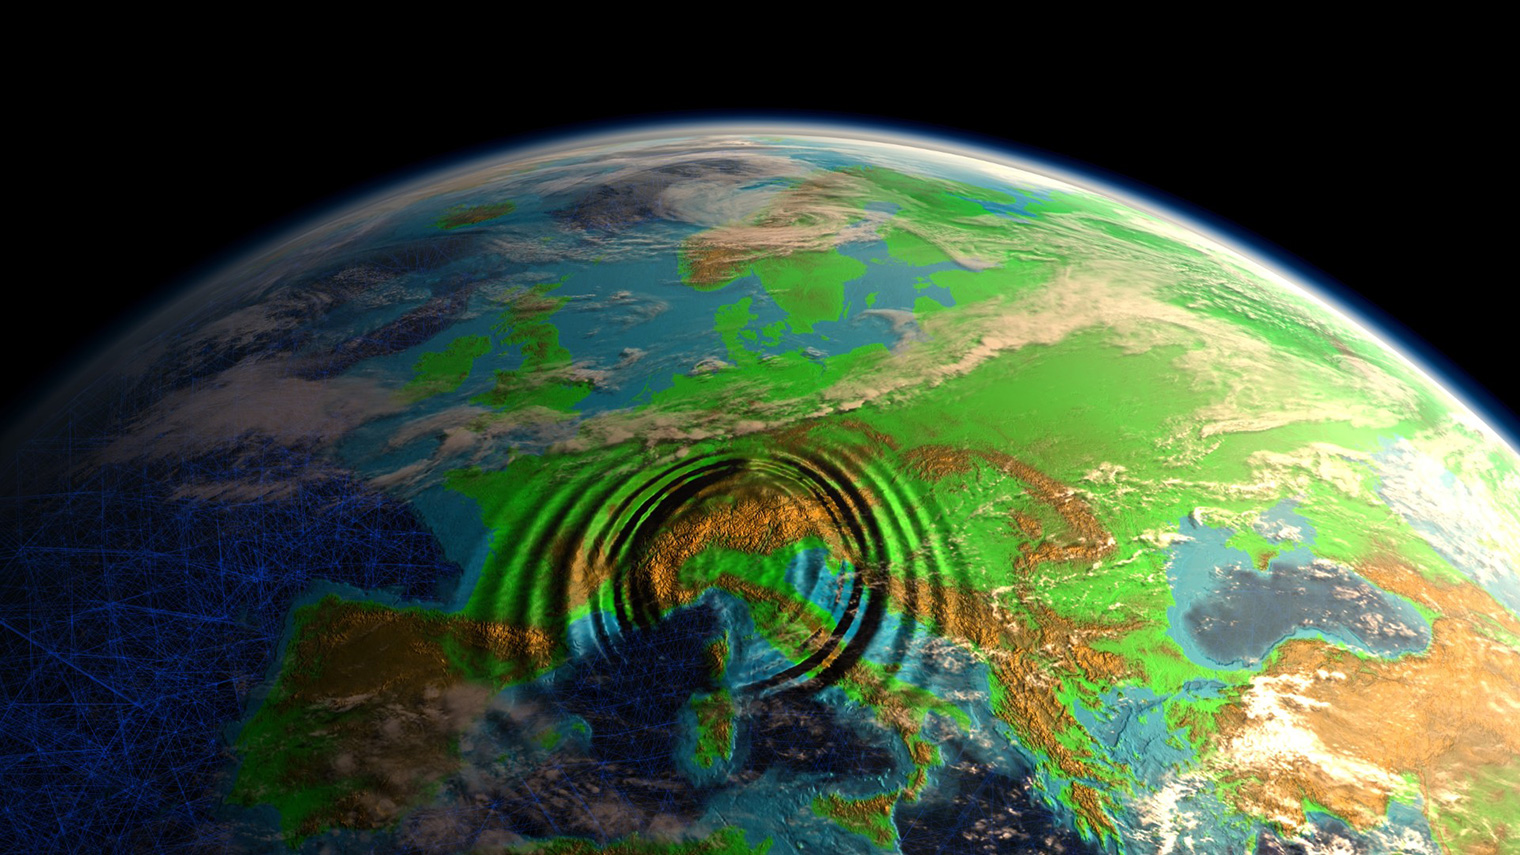
\includegraphics[width=\paperheight, height=\paperheight, keepaspectratio]{2/SwDS_poster_template/Edinburgh_poster/earthquake.jpg}}
}

% To use the framed environment 
\usepackage{framed} 

% Bibliography without title.
\usepackage[square, numbers, comma]{natbib}
\renewcommand{\bibsection}{}

% Caption for use outside floats.
\newcommand{\myCaption}[1]{\parbox{\linewidth}{\large \vspace{10pt} #1 \vspace{10pt}}}

% Subfigures, etc.
\usepackage{subfigure}

%\usepackage{pagegrid}
\usepackage{eucal}

% My maths macros.
%\usepackage{mathsMacros}

% Orange emphasis.
\newcommand{\oEmph}[1]{\textcolor{orange}{#1}}

% My commands.
\newcommand{\Exponential}{\mathrm{Exp}}
\newcommand{\diff}{\mathrm{d}}
\newcommand{\grad}{\nabla}
\newcommand{\Ind}{\mathbb{I}}
\newcommand{\Uniform}{\mathrm{Uniform}}
\newcommand{\lambdaref}{\lambda_{\text{ref}}}

%%%%%%%%%%%%%%%%%%%%%%%%%%%%%%%%%%%%%%%%%%%
%
% TIKZ packages and common definitions
%
% Add extra things as per your tikz needs
%
%%%%%%%%%%%%%%%%%%%%%%%%%%%%%%%%%%%%%%%%%%%

\usepackage{picins}
\usepackage{tikz}
\usetikzlibrary{shapes.geometric,arrows,chains,matrix,positioning,scopes,calc}
\tikzstyle{mybox} = [draw=white, rectangle]

\graphicspath{{PosterFigures/}{PaperFigures/}{Branding/}}

%%%%%%%%%%%%%%%%%%%%%%%%%%%%%%%%%%%%%%%%%%%
%
% Some standard colours
%
%%%%%%%%%%%%%%%%%%%%%%%%%%%%%%%%%%%%%%%%%%%

\definecolor{oxdarkblue}{cmyk}{1, 0.8, 0, 0.6}
\definecolor{lightblue}{rgb}{0, 0, 0.80}
\definecolor{white}{rgb}{1, 1, 1}
\definecolor{whiteblue}{rgb}{0.80, 0.80, 1}

%%%%%%%%%%%%%%%%%%%%%%%%%%%%%%%%%%%%%%%%%%%
%
% Some look and feel definitions
%
%%%%%%%%%%%%%%%%%%%%%%%%%%%%%%%%%%%%%%%%%%%

\setlength{\columnsep}{0.05\textwidth}
\setlength{\columnseprule}{0.00025\textwidth}
\setlength{\parindent}{1cm}
\setlength{\parskip}{1cm}

%%%%%%%%%%%%%%%%%%%%%%%%%%%%%%%%%%%%%%%%%%%
%
% \mysection - replacement for \section*
% 
%%%%%%%%%%%%%%%%%%%%%%%%%%%%%%%%%%%%%%%%%%%

\tikzstyle{mysection} = [rectangle, 
	draw=none, 
	shade, 
	outer color=oxdarkblue,
	inner color=oxdarkblue,
	text width=0.97\columnwidth,
	text centered,
	text=white,
	rounded corners=20pt,
	minimum height=3cm]%0.11\columnwidth]

\newcommand{\mysection}[1]
{
	\begin{center}
		\begin{tikzpicture}
			\node[mysection] {\sffamily\bfseries\LARGE#1};
		\end{tikzpicture}
	\end{center}
}


\newcommand{\mysubsection}[1]
{
			{\sffamily\bfseries#1}
}


%%%%%%%%%%%%%%%%%%%%%%%%%%%%%%%%%%%%%%%%%%%%
%%
%% \myalign - replacement for {align*}
%% 
%%%%%%%%%%%%%%%%%%%%%%%%%%%%%%%%%%%%%%%%%%%%
%
%\tikzstyle{myalign} = [draw, rectangle, 
%	text width=\columnwidth,
%	text centered,
%	text=black]
%
%\newcommand{\myalign}[1]
%{
%	\begin{center}
%		\begin{tikzpicture}
%			\node[myalign] {\Large $ \begin{aligned} #1 \end{aligned} $};
%		\end{tikzpicture}
%	\end{center}
%}

%%%%%%%%%%%%%%%%%%%%%%%%%%%%%%%%%%%%%%%%%%%
%
% Set the font
%
%%%%%%%%%%%%%%%%%%%%%%%%%%%%%%%%%%%%%%%%%%%

\renewcommand{\familydefault}{cmss}
\sffamily

%%%%%%%%%%%%%%%%%%%%%%%%%%%%%%%%%%%%%%%%%%%
%
% New commands on theorem and proofs 
%
%%%%%%%%%%%%%%%%%%%%%%%%%%%%%%%%%%%%%%%%%%%
\newcommand{\iid}{\overset{i.i.d.}{\sim}}


%%%%%%%%%%%%%%%%%%%%%%%%%%%%%%%%%%%%%%%%%%%
%
% Poster environment
%
%%%%%%%%%%%%%%%%%%%%%%%%%%%%%%%%%%%%%%%%%%%

\newenvironment{poster}
{
	\begin{center}
		\hspace{-2in}
		\begin{minipage}[c]{0.96\textwidth}
		}
		{
		\end{minipage} 
	\end{center}
}

%%%%%%%%%%%%%%%%%%%%%%%%%%%%%%%%%%%%%%%%%%%
%
% The document environment starts here
%
%%%%%%%%%%%%%%%%%%%%%%%%%%%%%%%%%%%%%%%%%%%

\begin{document}

%%%%%%%%%%%%%%%%%%%%%%%%%%%%%%%%%%%%%%%%%%%
%
% Begin the poster environment - centres things etc
%
%%%%%%%%%%%%%%%%%%%%%%%%%%%%%%%%%%%%%%%%%%%

\begin{poster}

\vspace{1\baselineskip}

%%%%%%%%%%%%%%%%%%%%%%%%%%%%%%%%%%%%%%%%%%%
%
% Draw the header as a TIKZ picture
%
%%%%%%%%%%%%%%%%%%%%%%%%%%%%%%%%%%%%%%%%%%%

\nocite{vanetti2017piecewise}

\begin{center}
	\begin{tikzpicture}
		\begin{scope}

			\node[inner sep=0, text width=0.64\textwidth, text centered, anchor=north west, font=\Huge] (Title) at (0, 0) 
			{
				{\sffamily
                                  \Huge \textbf{Mimicking L'Aquila: Capturing Key Components of the Earthquake Sequence} \\
                                } 
				{\sffamily\huge    Robin Lin*\\                  
 \sffamily  Supervisors: Dr. Finn Lindgren and Dr. Daniel Paulin}\\

 {\LARGE \texttt{*Tel: +44 (0)7536141692, Email: s2435943@ed.ac.uk}}
			};


                        \node[mybox, anchor=north west] (box) at ($(Title.north east) + (0, 0 em) $)
                        {
                          
\includegraphics[width=0.32\textwidth]{Branding/Mathematics_2col_cmyk.eps}
                        };

                
		\end{scope}
	\end{tikzpicture}
\end{center}

%%%%%%%%%%%%%%%%%%%%%%%%%%%%%%%%%%%%%%%%%%%
%
% Spacing between title and main body
%
%%%%%%%%%%%%%%%%%%%%%%%%%%%%%%%%%%%%%%%%%%%

%\vspace{2\baselineskip}
%\vspace{1\baselineskip} % Add this back in!

%%%%%%%%%%%%%%%%%%%%%%%%%%%%%%%%%%%%%%%%%%%
%
% Main body
%
%%%%%%%%%%%%%%%%%%%%%%%%%%%%%%%%%%%%%%%%%%%

\Large % this gives the font size, for detail see: http://www.ctex.org/documents/packages/nonstd/a0poster.pdf


\begin{tikzpicture}
\begin{scope}

\node (n1) [text width=0.48\textwidth, align = justify, anchor = north west, inner sep = 0] at (3em, 0)
{

\mysection{Overview}

This project aims at mimicking the L'Aquila earthquake sequence using synthetic catalogues, and investigating catalogue characteristics in order to yield a better performance in resembling the real sequence.
};


\node (n1b) [text width=0.48\textwidth, align = justify, anchor = north west, inner sep = 0] at ($(n1.south west) + (0, 0) $)
{

\mysection{L'Aquila Sequence}

\begin{minipage}[l]{.5\textwidth}
\textbf{Map Description}\\
This map illustrates vividly the locations of Italian earthquakes in $2009$. Different colours of dots show different magnitudes.
\begin{itemize}
    \item Black: Richter scale of $3$ to $5$
    \item Orange: Richter scale of $5$ to $6$
    \item Red: The L'Aquila earthquake, Richter scale of $6.29$
\end{itemize} 
\textbf{Earthquake Characteristics}
\begin{itemize}
    \item Number of events: $1024$ (Richter scale of at least $M_0=2.5$)
    \item Number of large events (Richter scale of $4.5$ or higher): $14$
    \item Largest event: Richter scale of $6.29$
\end{itemize} 

\end{minipage}
\hfill
\begin{minipage}[c]{.5\textwidth}

\begin{center}
\transparent{0.7}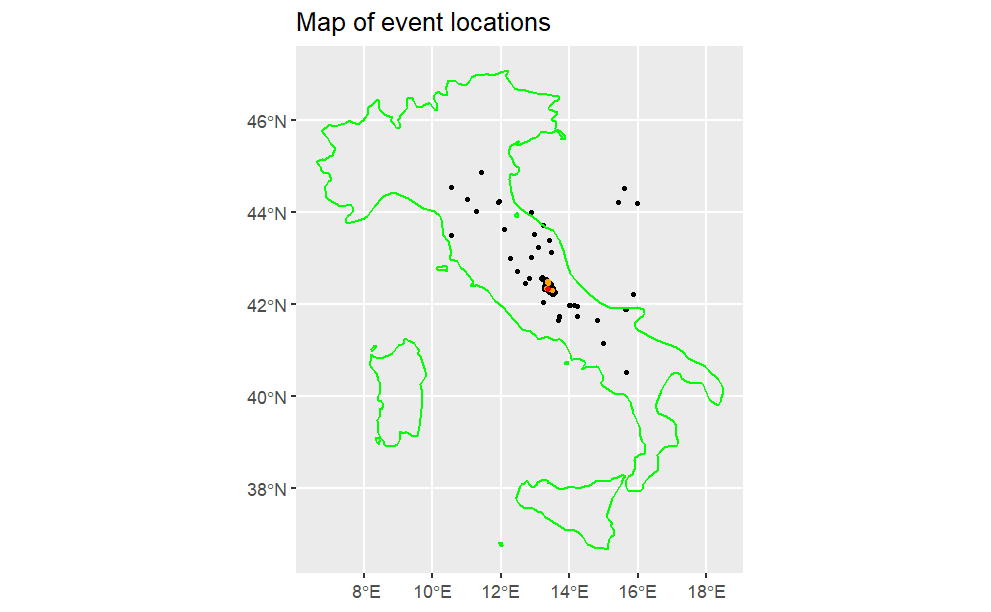
\includegraphics[width=\linewidth]{2/MSc_LaTeX_SwDS/MSc_LaTeX_SwDS/Italy.png}\\
\scriptsize Figure 1. \textbf{Locations of Earthquakes in Italy, $2009$}
\end{center}
\end{minipage}
};

\node (n1c) [text width=0.48\textwidth, align = justify, anchor = north west, inner sep = 0] at ($ (n1b.south west) + (0, 0) $)
{
\mysection{Modelling the Sequence}
\begin{minipage}[l]{.5\textwidth}
\begin{center}
\transparent{0.7}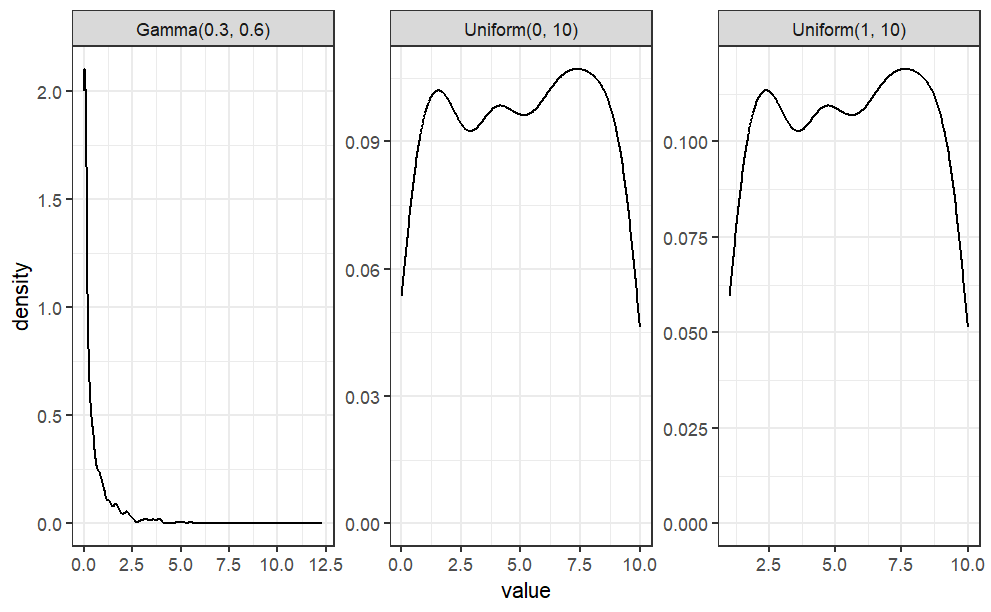
\includegraphics[width=\linewidth]{2/MSc_LaTeX_SwDS/MSc_LaTeX_SwDS/prior_orig}\\
\scriptsize Figure 2. \textbf{Prior Distributions of the Parameters}

\transparent{0.7}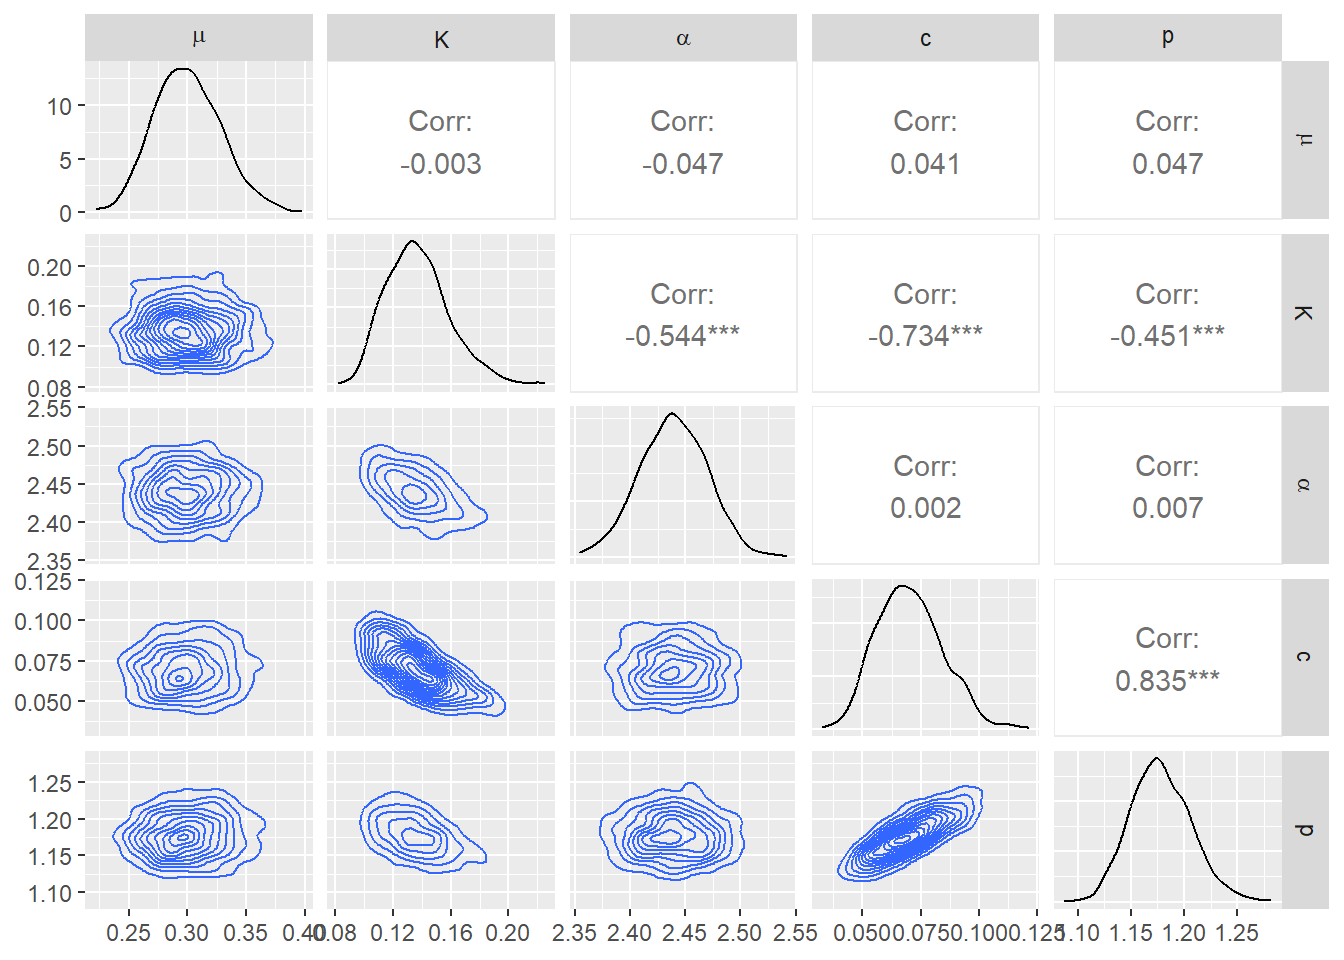
\includegraphics[width=\linewidth]{2/MSc_LaTeX_SwDS/MSc_LaTeX_SwDS/pairplot.png}\\
\scriptsize Figure 3. \textbf{Posterior Parameter Estimations of the L'Aquila Sequence}
\end{center}
\end{minipage}
\hfill
\begin{minipage}[c]{.5\textwidth}
According to \cite{serafini2023approximation} \cite{naylor2023bayesian}, the Epidemic Type Aftershock Sequence (ETAS) model is adopted to estimate $5$ parameters.
\begin{itemize}
\item $\mu$, background rate. Prior distribution: $Gamma(0.3, 0.6)$.
\item $K$, productivity, mean aftershocks. Prior distribution: $U(0, 10)$.
\item $\alpha$, magnitude scales, changes in aftershocks given an earthquake event. Prior distribution: $U(0, 10)$.
\item $c$, time offset, positively correlated to missing events. Prior distribution: $U(0, 10)$.
\item $p$, decaying rate of aftershocks. Prior distribution: $U(1, 10)$.
\end{itemize}
The posterior distributions of the $5$ parameters are then sketched in Figure 3.
\end{minipage}
\hfill
\begin{minipage}[l]{.5\textwidth}
%\textbf{Sensitivities of Parameters}
\begin{itemize}
\item Mis-specifying prior of $\mu$ to be $Gamma(5, 1)$, or that of $\alpha$ to be $U(0.99, 1.01)$, no effects on posterior results.
\item Mis-specifying prior of $K$ or $c$ to be $U(0.99,1.01)$, or that of $p$ to be $U(4.9, 5.1)$, significant effects on posterior results.
\end{itemize}
%Priors of $K, c, p$ are to be correctly specified in order to obtain the true distributions of other parameters.
\end{minipage}
\hfill
\begin{minipage}[c]{.5\textwidth}
\begin{center}
\transparent{0.7}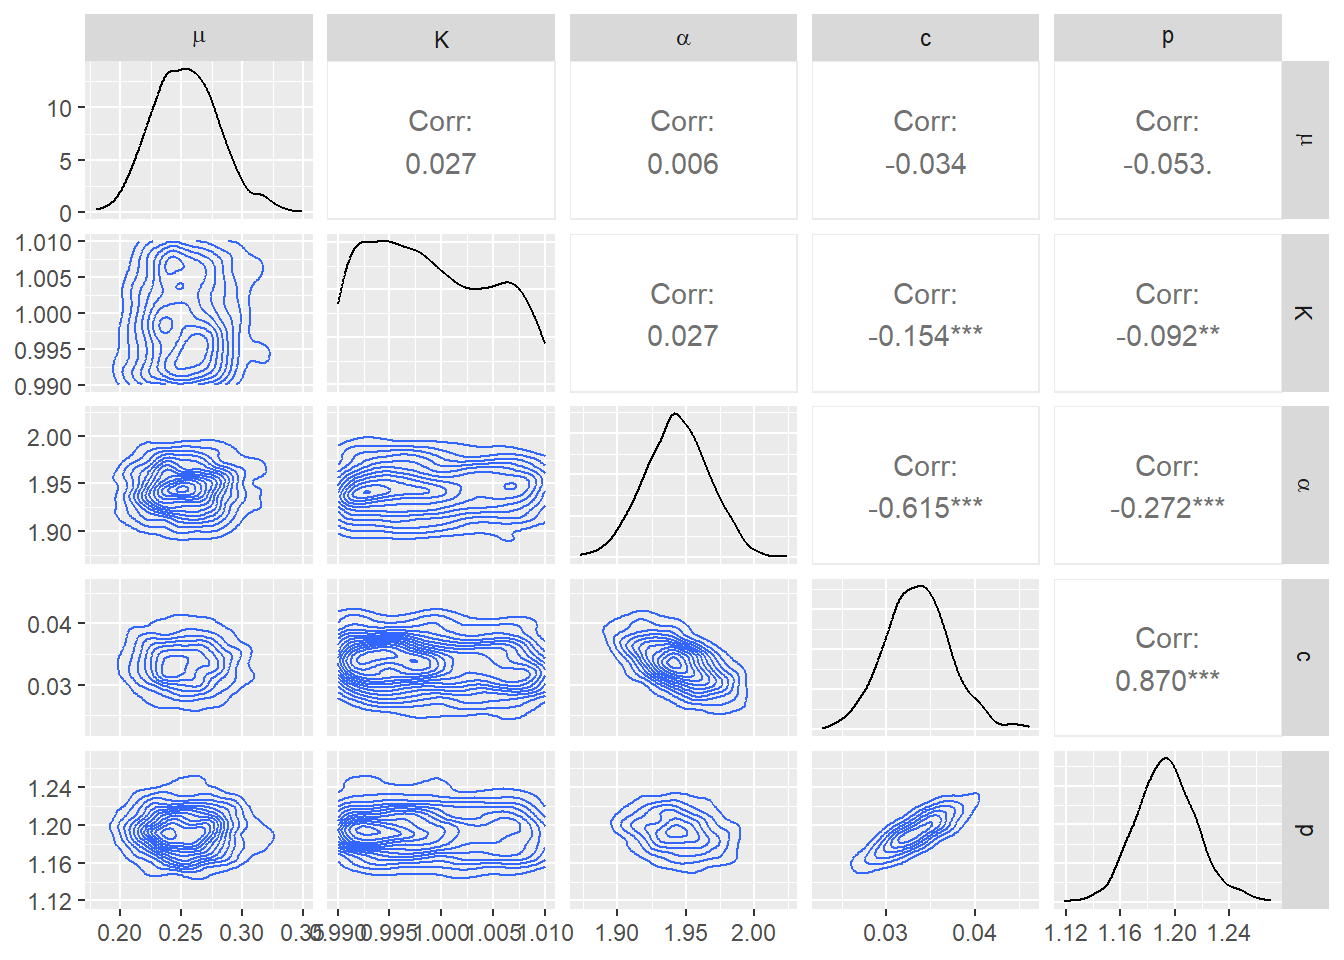
\includegraphics[width=\linewidth]{2/MSc_LaTeX_SwDS/MSc_LaTeX_SwDS/pairplot_K.png}\\
\scriptsize Figure 4. \textbf{Posterior Parameter Distributions, mis-specifying $K$}
\end{center}
\end{minipage}
\hfill
\begin{minipage}[l]{.5\textwidth}
\begin{center}
\transparent{0.7}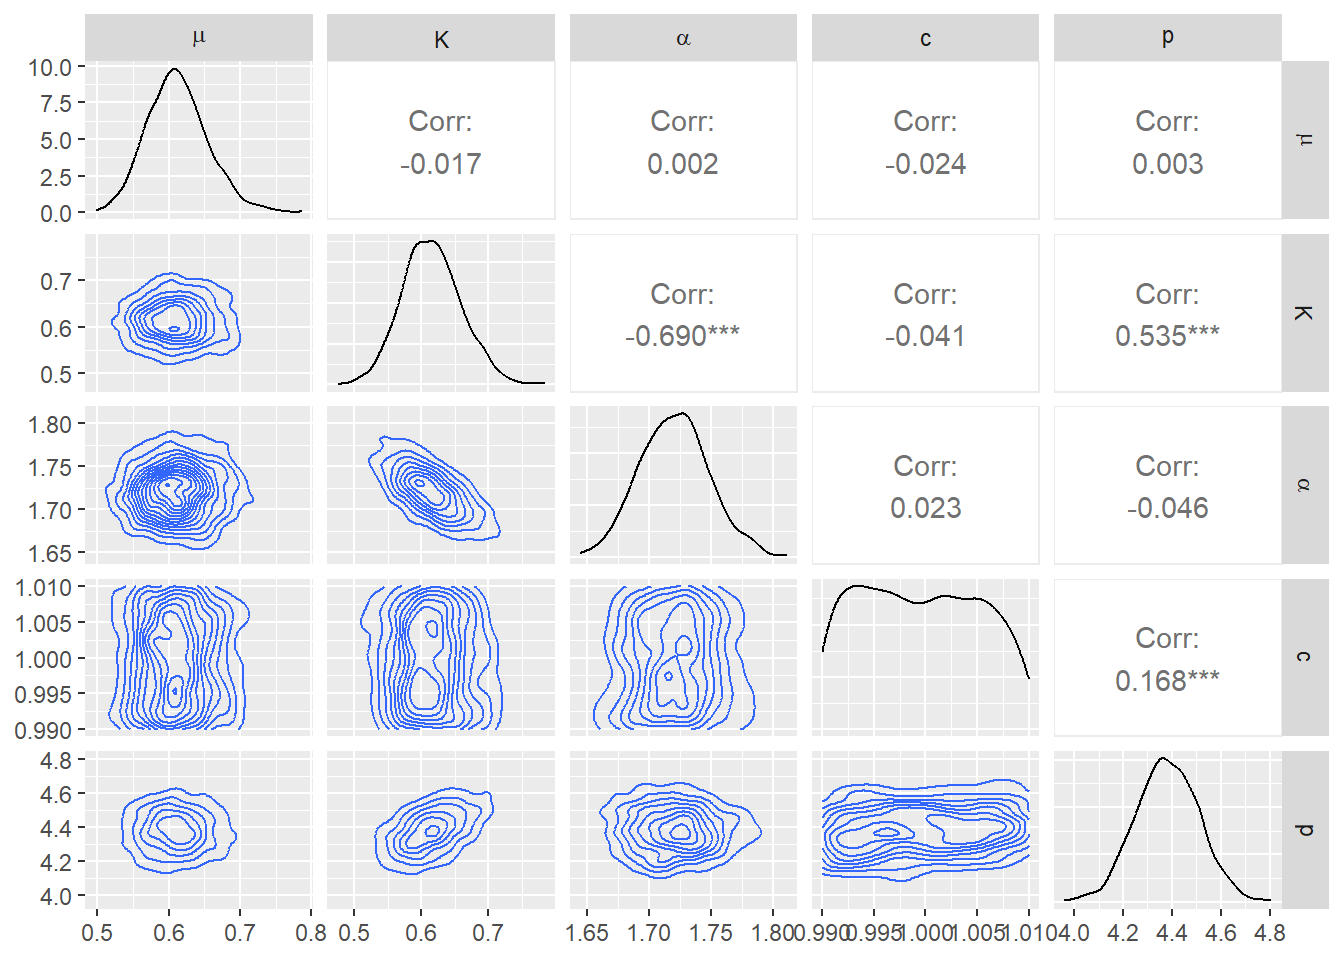
\includegraphics[width=\linewidth]{2/MSc_LaTeX_SwDS/MSc_LaTeX_SwDS/pairplot_c.png}\\
\scriptsize Figure 5. \textbf{Posterior Parameter Distributions, mis-specifying $c$}
\end{center}
\end{minipage}
\hfill
\begin{minipage}[l]{.5\textwidth}
\begin{center}
\transparent{0.7}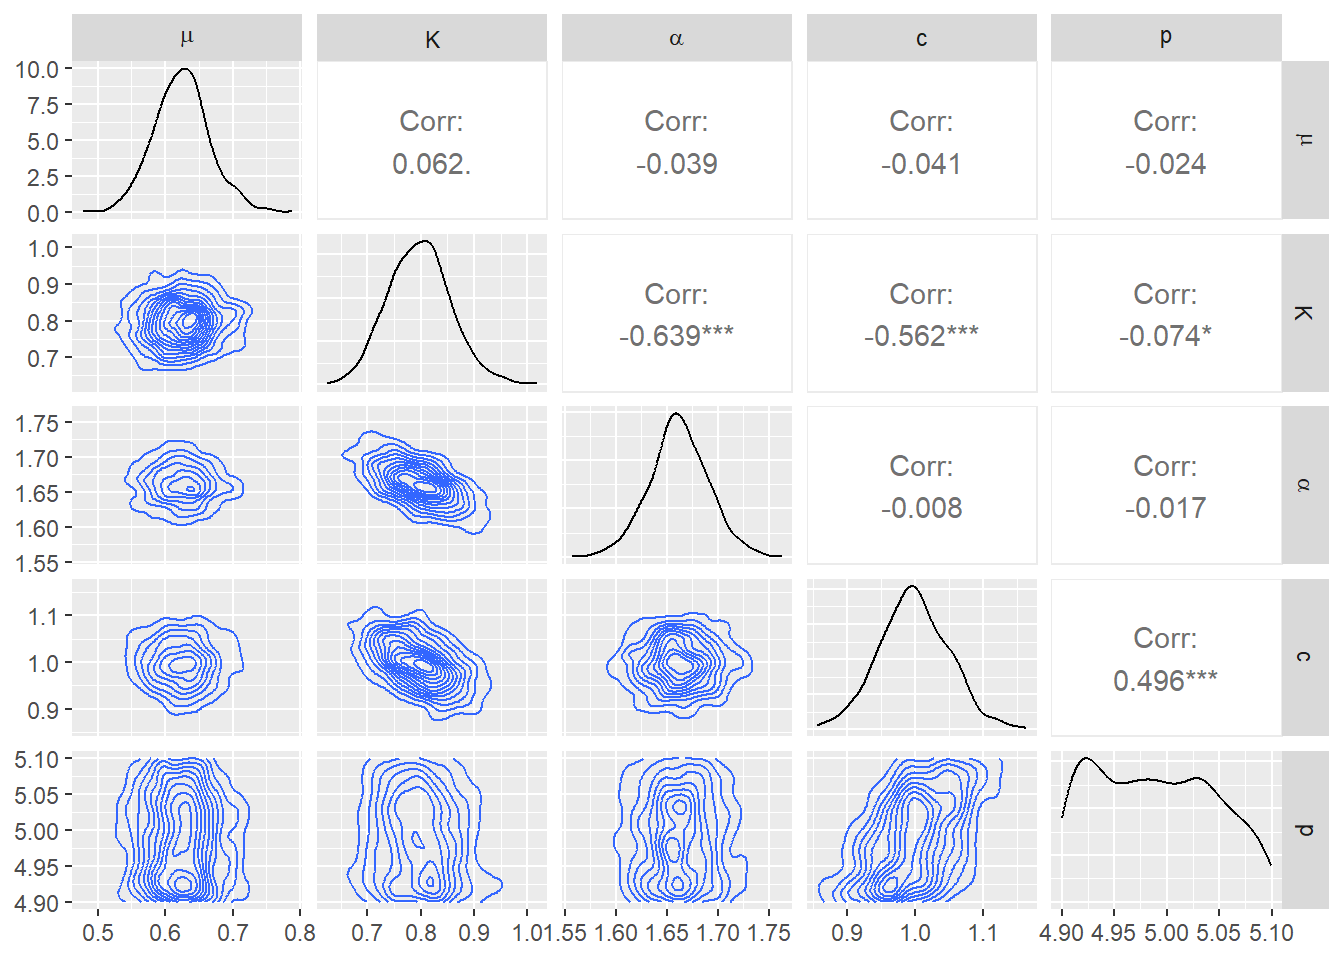
\includegraphics[width=\linewidth]{2/MSc_LaTeX_SwDS/MSc_LaTeX_SwDS/pairplot_p.png}\\
\scriptsize Figure 6. \textbf{Posterior Parameter Distributions, mis-specifying $p$}
\end{center}
\end{minipage}

};


\node (n20) [text width=0.48\textwidth, align = justify, anchor = north west, inner sep = 0] at ($ (n1.north east) + (2em, 0) $)
{
	\mysection{Generating and Modelling the Synthetic Catalogues}
\begin{minipage}[l]{.6\textwidth}
$1000$ synthetic catalogues are generated, without imposing history (to avoid generating an unrealistically large amount of catalogues), with parameter values specified in the table.
\end{minipage}
\hfill
\begin{minipage}[c]{.4\textwidth}
\centering
\begin{tabular}{|c|c|c|c|c|c|}

\hline
$\mu$   & K    & $\alpha$  & c    & p    & $\beta$ \\ \hline
0.30 & 0.14 & 2.44 & 0.07 & 1.18 & 2.35 \\ \hline

\end{tabular}\\
\scriptsize Table. \textbf{Parameter Values for Synthetic Catalogues}\\

\normalsize
$\beta$: magnitude distribution parameter, \\
$\hat \beta = \frac{1}{mean(magnitudes)-M_0}$.
\end{minipage}
\hline
\begin{minipage}[l]{.5\textwidth}
\begin{center}
\transparent{0.7}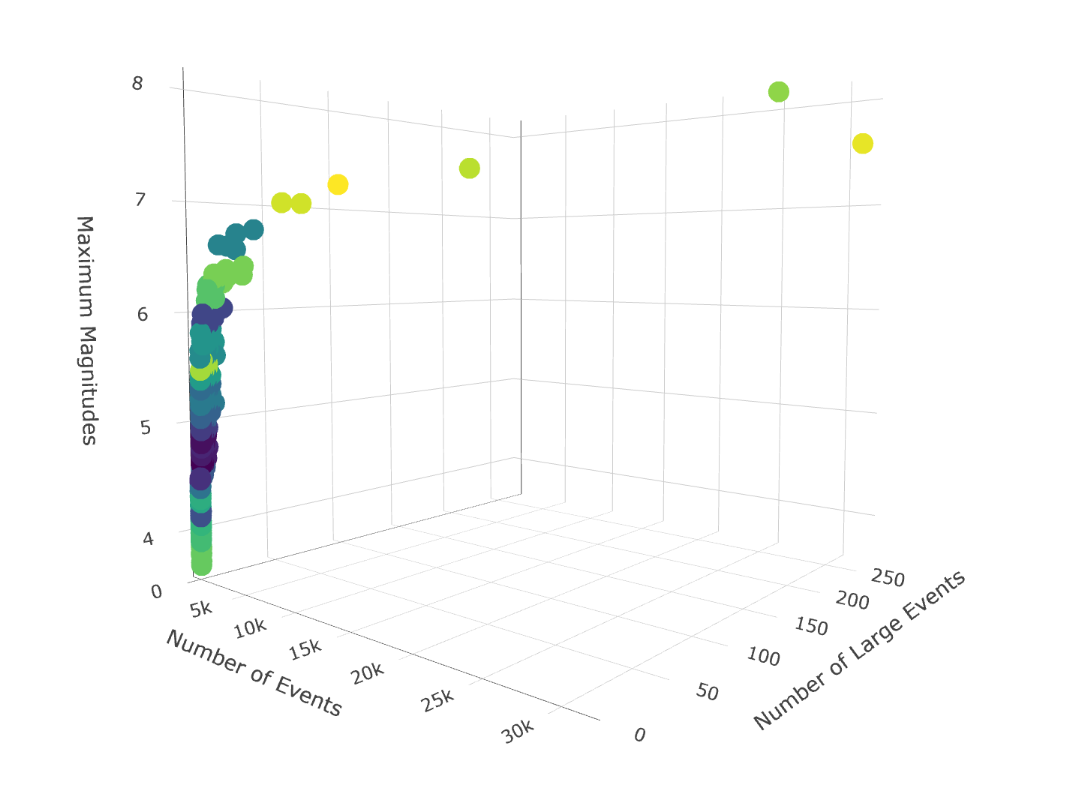
\includegraphics[scale = 1]{2/MSc_LaTeX_SwDS/MSc_LaTeX_SwDS/cluster3d.png}\\
\scriptsize Figure 7. \textbf{Clustered $3D$ Characteristic Scatter Plot}
\end{center}
\end{minipage}
\hfill
\begin{minipage}[c]{.5\textwidth}
Catalogues are recursively grouped into $25$ clusters based on their characteristics using hierarchical clustering. Dendrogram and clustered $3D$ characteristic scatter plot are shown.
\begin{center}
\transparent{0.7}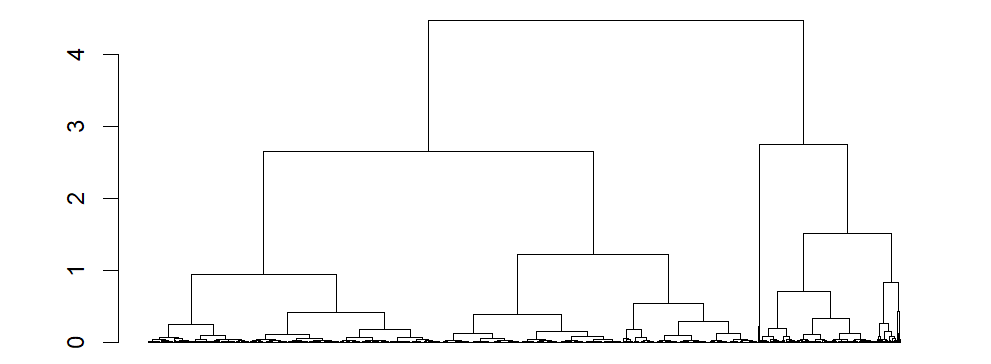
\includegraphics[scale = 1]{2/MSc_LaTeX_SwDS/MSc_LaTeX_SwDS/dendro.png}\\
\scriptsize Figure 8. \textbf{Dendrogram}
\end{center}
\end{minipage}
\hline
\begin{minipage}[l]{\textwidth}
$1$ catalogue from each cluster is selected, and the ETAS model is applied to these catalogues. $2$ of the posterior plots are shown.
\end{minipage}
\hfill
\begin{minipage}[c]{.5\textwidth}
\begin{center}
\transparent{0.7}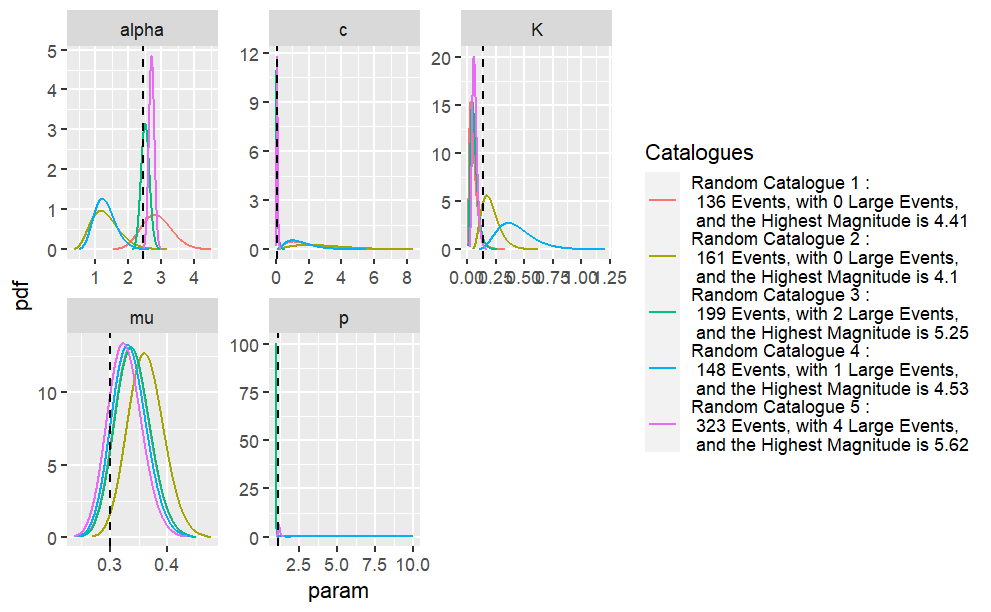
\includegraphics[width = \textwidth]{2/MSc_LaTeX_SwDS/MSc_LaTeX_SwDS/synfit3.png}\\
\scriptsize Figure 9. \textbf{Posterior Plot $(1)$}
\end{center}
\end{minipage}
\hfill
\begin{minipage}[c]{.5\textwidth}
\begin{center}
\transparent{0.7}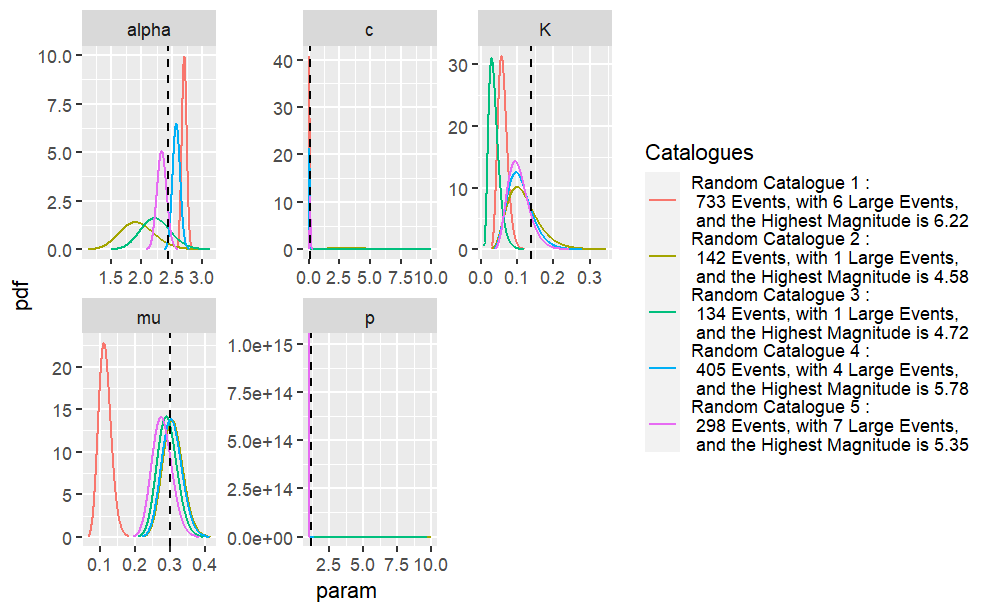
\includegraphics[width = \textwidth]{2/MSc_LaTeX_SwDS/MSc_LaTeX_SwDS/synfit4.png}\\
\scriptsize Figure 10. \textbf{Posterior Plot $(2)$}
\end{center}
\end{minipage}
\hline
Organic synthetic catalogues (no history imposed) with $200$ to $400$ total events, with $3$ to $5$ large events, and with the largest event of magnitude around $6$ would lead to a better performance in estimating the parameters.	
};

\node (n21) [text width=0.48\textwidth, align = justify, anchor = north west, inner sep = 0] at ($(n20.south west) + (0, 0) $)
{
\mysection{Investigating Time-between-Events}
\textbf{Organic Synthetic Catalogues}

\begin{minipage}[l]{.5\textwidth}
\begin{center}
\transparent{0.7}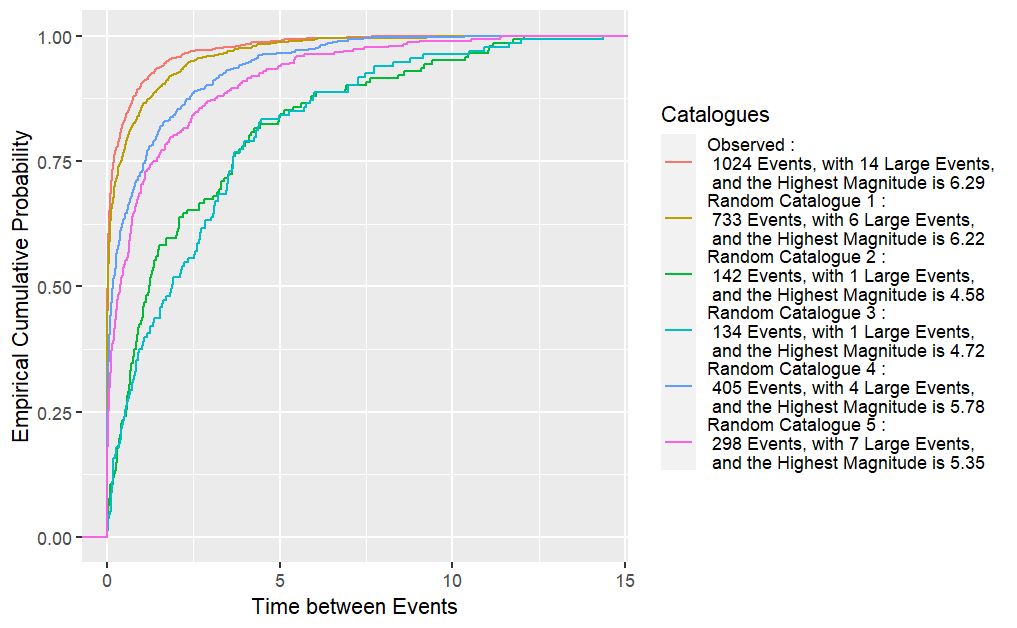
\includegraphics[width = \textwidth]{2/MSc_LaTeX_SwDS/MSc_LaTeX_SwDS/ecdf4.png}\\
\scriptsize Figure 11. \textbf{Empirical Distributions of Time-between-Events}
\end{center}
\end{minipage}
\hfill
\begin{minipage}[c]{.5\textwidth}
\begin{center}
\transparent{0.7}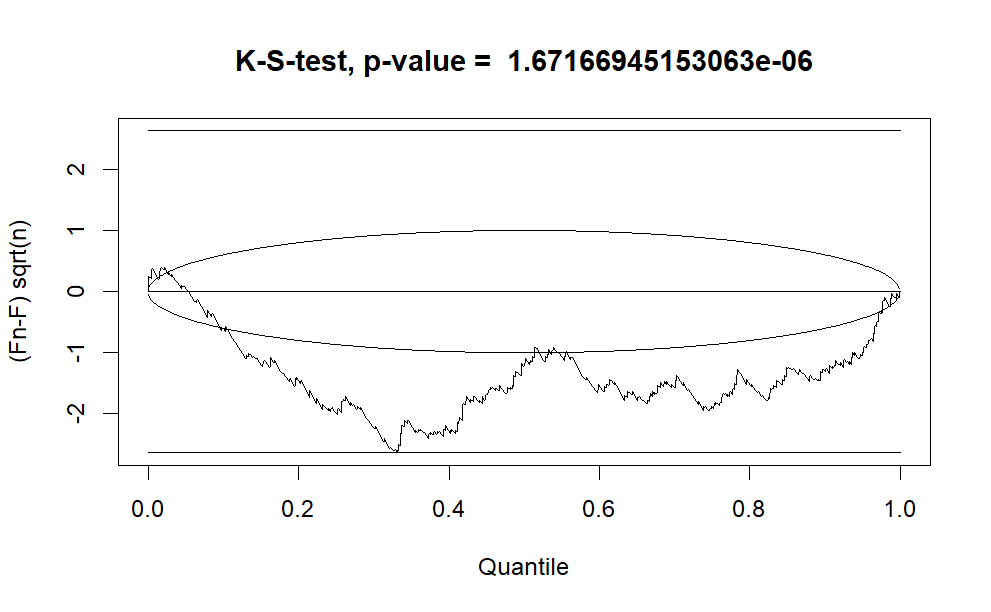
\includegraphics[width = \textwidth]{2/MSc_LaTeX_SwDS/MSc_LaTeX_SwDS/ks_org_best.png}\\
\scriptsize Figure 12. \textbf{An Example Kolmogorov-Smirnov Test Plot}
\end{center}
\end{minipage}
\hline
\textbf{Synthetic Catalogues with L'Aquila Earthquake Imposed}

\begin{minipage}[l]{.5\textwidth}
\begin{center}
\transparent{0.7}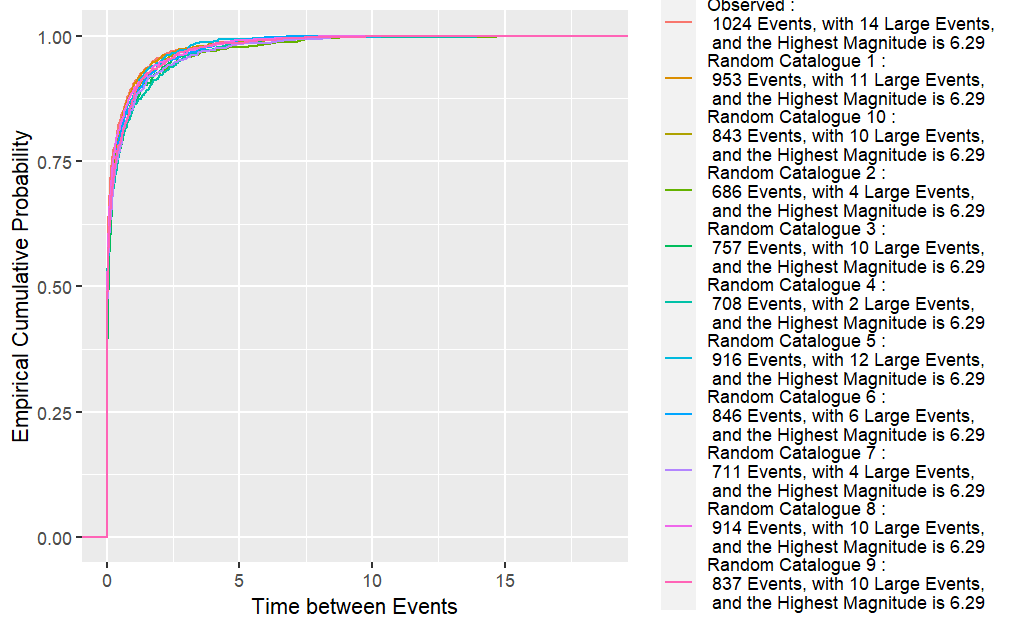
\includegraphics[width = \textwidth]{2/MSc_LaTeX_SwDS/MSc_LaTeX_SwDS/ecdf_imp.png}\\
\scriptsize Figure 13. \textbf{Empirical Distributions of Time-between-Events}
\end{center}
\end{minipage}
\hfill
\begin{minipage}[c]{.5\textwidth}
\begin{center}
\transparent{0.7}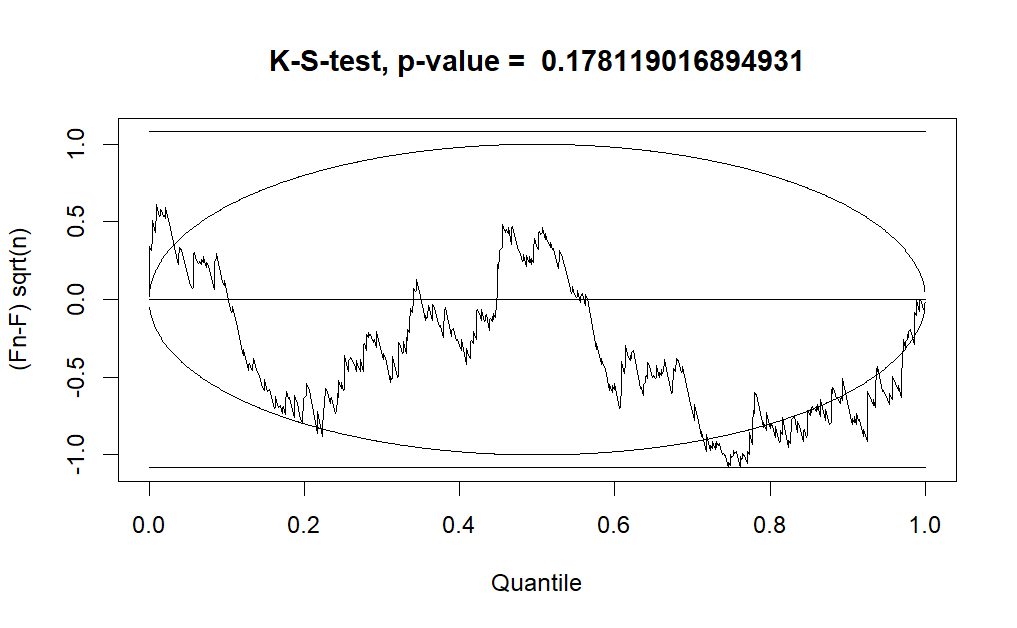
\includegraphics[width = \textwidth]{2/MSc_LaTeX_SwDS/MSc_LaTeX_SwDS/ks_imp_best.png}\\
\scriptsize Figure 14. \textbf{An Example Kolmogorov-Smirnov Test Plot}
\end{center}
\end{minipage}
\hline
When investigating time differences between $2$ consecutive events, imposing the main event to the history will increase the chance of generating catalogues having similar number of events, similar number of large events, as well as the similar highest magnitude with the real L'Aquila sequence, yielding a better performance in simulating the arrival time of the earthquakes. However, this does not necessarily mean that imposing events will lead to better estimates of the $5$ parameters specified above, which is the reason why events are only imposed to the history when the inter-arrival periods are to be simulated.

};


\node (n22) [text width=0.48\textwidth, align = justify, anchor = north west, inner sep = 0] at ($ (n21.south west)$)
{
\mysection{Main References}

{
%	You can include your bibliography in a bib file here
%\normalsize
%\bibliographystyle{apalike}
%\bibliography{2/SwDS_poster_template/Edinburgh_poster/literature}


\footnotesize % Reduce the font size in this block
%\renewcommand{\section}[2]{\vskip 0.01em} % Get rid of the default "References" section title
%\nocite{Hill1995} % Insert publications even if they are not cited in the poster
\bibliographystyle{unsrt}
\bibliography{literature} % Use sample.bib as the bibliography file

}

};

%%%%%%%%%%%%%%%%%%%%%%%%%%%%%%%%%%%%%%%%%%%
%
% Decorative lines.
%
%%%%%%%%%%%%%%%%%%%%%%%%%%%%%%%%%%%%%%%%%%%



% this is a separating line between  the two text columns
\node (l1) at ($ (n1.north east) + (1em, 0) $) {};
\node (l2) at ($ (n1c.south east) + (1em, 0) $) {};
\draw[black] (l1) -- (l2);


%\node (l3) at ($ (n7.north east) + (0.025\linewidth, 0) $) {};
%\node (l4) at ($ (l2) + (0.35\linewidth, 0) $) {};
%\draw[black] (l3) -- (l4);


\end{scope}
\end{tikzpicture}

\end{poster}

\end{document}
